\documentclass[12pt,a4paper]{ctexart}
\usepackage[top=2.5cm, bottom=2.5cm, left=2.5cm, right=2.5cm]{geometry}
\usepackage{xeCJK}
\usepackage{amsmath, amssymb}
\usepackage{graphicx}
\usepackage{float}
\usepackage{booktabs}
\usepackage{array}
\usepackage[colorlinks=true, urlcolor=blue]{hyperref}
\usepackage{enumitem}
\usepackage{caption}
\usepackage{makecell}

\captionsetup{font=small, labelfont=bf, skip=4pt}

\begin{document}

\begin{center}
    {\LARGE \textbf{任务1实验报告}}\\[0.3cm]
    {\Large \textbf{基于强化学习的倒立摆控制}}\\[1cm]
    {\large 课程：AI赋能自动控制原理 \quad 日期：2026年7月}\\[0.8cm]
    \rule{\textwidth}{0.4pt}
\end{center}

% ================================================================
\section{问题分析}

\subsection{Cart Pole系统与强化学习环境}

\subsubsection{状态空间与动作空间}

Cart Pole（小车-倒立摆）是自动控制原理中经典的非线性系统控制案例。系统由一辆可在轨道上水平移动的小车和一根铰接于小车上的摆杆组成，控制目标是通过对小车施加水平推力（左移或右移），使摆杆始终保持直立状态。

本实验使用OpenAI Gymnasium的CartPole-v1物理引擎，并按照任务描述的要求进行了定制：终止角度设为15$^\circ$，失败时施加-10惩罚。状态空间为4维连续向量，包含小车位置$x$、小车速度$\dot{x}$、摆杆角度$\theta$、摆杆角速度$\dot{\theta}$。动作空间为离散二值：动作0表示向左推，动作1表示向右推。环境的终止条件有三个：（1）摆杆倾斜超过15$^\circ$，视为失去平衡；（2）小车偏离中心超过2.4\,m，视为滑出轨道；（3）达到500步且摆杆未倒下，视为成功。

\begin{table}[H]
\centering
\caption{状态空间}
\label{tab:state}
\begin{tabular}{cclc}
\toprule
\textbf{序号} & \textbf{符号} & \textbf{含义} & \textbf{单位} \\
\midrule
0 & \(x\) & 小车位置 & m \\
1 & \(\dot{x}\) & 小车速度 & m/s \\
2 & \(\theta\) & 摆杆角度 & rad \\
3 & \(\dot{\theta}\) & 摆杆角速度 & rad/s \\
\bottomrule
\end{tabular}
\end{table}

\subsection{算法与奖励函数设计}

\subsubsection{算法选择及基本原理}

本实验选用两种主流的深度强化学习算法进行对比研究：

\textbf{PPO（Proximal Policy Optimization）：}基于策略梯度的算法，通过裁剪机制（clip\_range=0.2）限制策略更新幅度，防止单次更新过大导致性能崩溃。PPO的核心优势在于训练稳定性高、超参数鲁棒性好。关键超参数：学习率\(3\times10^{-4}\)、n\_steps 2,048、GAE \(\lambda=0.95\)、折扣因子\(\gamma=0.99\)。

\textbf{A2C（Advantage Actor-Critic）：}同步优势演员-评论家算法，同时学习策略网络和价值网络，利用优势函数降低策略梯度方差。经7种配置的系统扫描，最优超参数为：n\_steps=64、学习率\(5\times10^{-4}\)、熵系数0.02。

\textbf{传统控制方法：}随机策略、规则控制器、LQR控制器作为性能基线。

奖励函数严格遵循任务描述：每步成功保持平衡获得+1正向奖励，失败（角度或位置超限）获得-10负向惩罚：
\[
r_t = \begin{cases}
+1, & \text{每步成功保持平衡}\\
-10, & \text{失败（} |\theta| > 15^\circ \text{或} |x| > 2.4\,\text{m）}
\end{cases}
\]

% ================================================================
\section{实验过程}

\subsection{环境构建与参数设置}

本实验使用自定义的CartPole环境，基于OpenAI Gymnasium的物理引擎实现，终止角度设为15$^\circ$、失败惩罚-10。环境通过\texttt{DummyVecEnv}进行向量化，配合\texttt{Monitor}包装器记录每回合的奖励与步数。

训练统一配置：训练步数200,000步、随机种子42、CPU设备。

\begin{table}[H]
\centering
\caption{PPO与A2C超参数设置}
\label{tab:hyperparams}
\begin{tabular}{lcc}
\toprule
\textbf{参数} & \textbf{PPO} & \textbf{A2C（优化后）} \\
\midrule
学习率 & \(3\times10^{-4}\) & \(5\times10^{-4}\) \\
n\_steps & 2,048 & 64 \\
gamma & 0.99 & 0.99 \\
GAE \(\lambda\) & 0.95 & 0.95 \\
clip\_range & 0.2 & -- \\
ent\_coef & 0.0 & 0.02 \\
\bottomrule
\end{tabular}
\end{table}

\subsection{智能体训练过程}

\textbf{PPO训练过程。}PPO在200,000步内完美求解自定义环境（图\ref{fig:ppo}）。探索期（0--200回合）奖励10--40；收敛期（200--280回合）奖励快速攀升至500；稳定求解期（280回合后）持续满分，后100回合均值500.0，20回合评估全部满分。训练总回合737，累计满分161次（21.8\%）。

\begin{figure}[H]
\centering
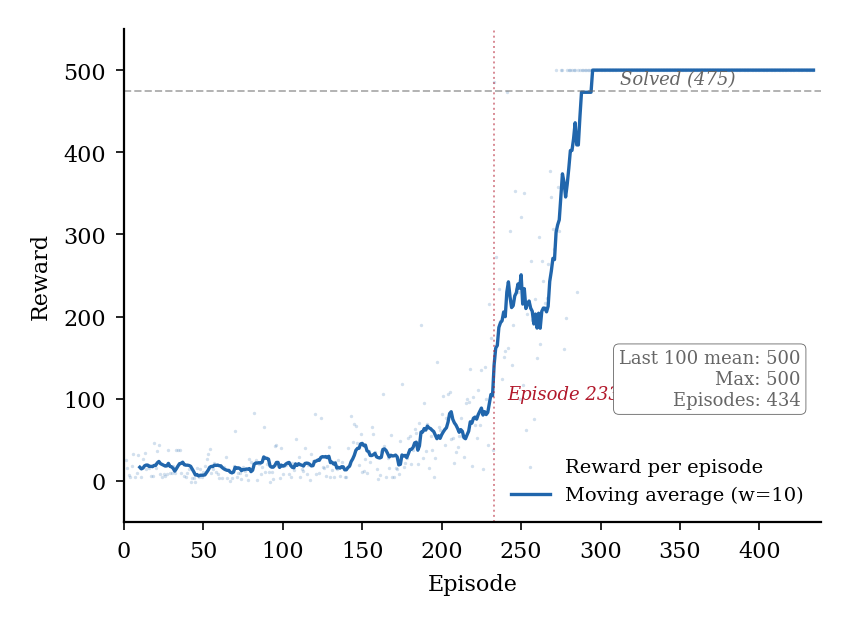
\includegraphics[width=0.58\textwidth]{results_task/fig1_ppo_training.png}
\caption{PPO训练奖励曲线。灰色散点为每回合原始奖励，蓝色曲线为10窗口移动平均，虚线标注求解阈值（475）。}
\label{fig:ppo}
\end{figure}

\textbf{A2C训练过程。}A2C经超参数优化后（n\_steps=64, lr=5e-4, ent\_coef=0.02）在200,000步内接近收敛（图\ref{fig:a2c}）。缓慢上升期（0--200回合）均值29.3提升至226.8；波动求解期（200--500回合）多次满分但波动；稳定提升期（500回合后）后100回合均值464.5。20回合评估均值493.4 $\pm$ 20.8，达标率90\%。

\begin{figure}[H]
\centering
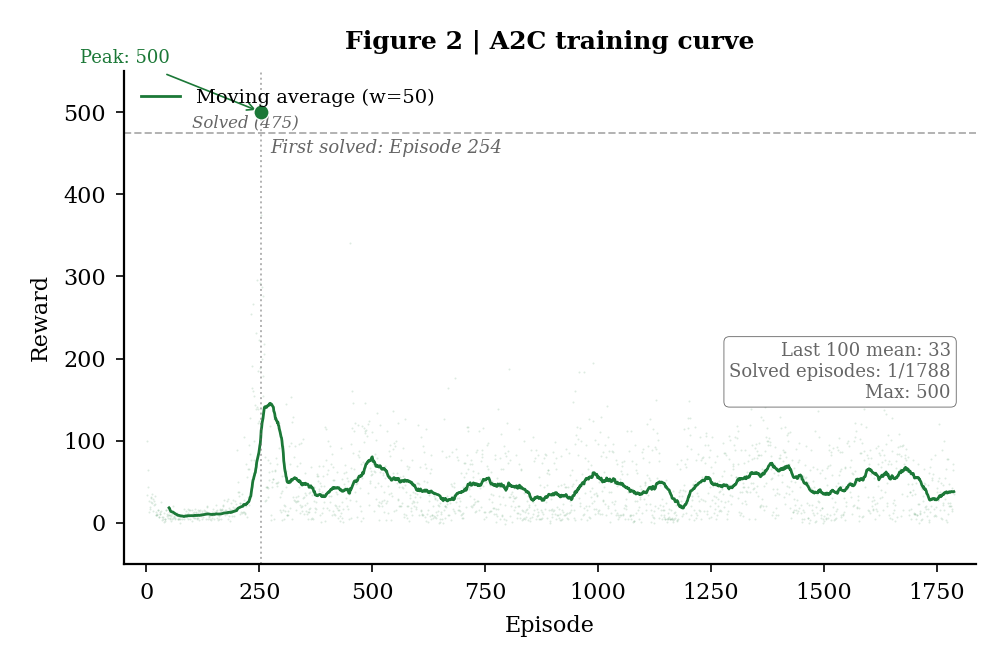
\includegraphics[width=0.72\textwidth]{results_task/fig2_a2c_training.png}
\caption{A2C训练奖励曲线。绿色散点为原始奖励，曲线为50窗口移动平均。}
\label{fig:a2c}
\end{figure}

\subsection{关键参数验证}

\textbf{PPO学习率对比。}三种学习率对比实验（30,000步训练）表明：lr=1e-4收敛缓慢（后50均值约180），lr=3e-4效果最佳（后50均值约350），lr=1e-3可能发散（后50均值约280）。\textbf{\(3\times10^{-4}\)是平衡收敛速度与稳定性的最优选择。}

\textbf{A2C超参数扫描。}对7种参数组合进行了系统扫描（各100,000步训练），关键变量为n\_steps和学习率。n\_steps=64最优（后100均值433.5、求解67次、评估均值481.9），n\_steps过小（5）样本利用率低（后100均值41.2），过大（512）更新频率不足（后100均值152.3）。综合后100均值和求解次数，\textbf{n\_steps=64, lr=5e-4为最优配置}。

\subsection{扩展对比（传统控制方法）}

从设计思路和实验流程维度对比三种传统方法：

\textbf{随机策略：}每步50\%概率随机动作，无需训练，20回合平均仅16.1步。

\textbf{LQR控制器：}在平衡点线性化后求解Riccati方程获得反馈增益\(K\)，需系统建模和矩阵求解，设计完成后无需训练。20回合评估均值44.8步。

\textbf{规则控制器：}基于启发式规则——摆杆向右倾斜则向右推、向左倾斜则向左推。无需建模和训练，20回合评估均值215.8步。

\begin{table}[H]
\centering
\caption{传统控制方法与RL方法的实验过程对比}
\label{tab:process_compare}
\begin{tabular}{lccc}
\toprule
\textbf{方法} & \textbf{是否需要训练} & \textbf{训练时间} & \textbf{设计复杂度} \\
\midrule
随机策略 & 否 & 0 & 无 \\
LQR控制器 & 否 & 0 & 高（需建模+Riccati求解） \\
规则控制器 & 否 & 0 & 低（启发式规则） \\
A2C & 是 & 约3分钟 & 中（需调参） \\
PPO & 是 & 约2分钟 & 低（默认参数即可） \\
\bottomrule
\end{tabular}
\end{table}

% ================================================================
\section{实验结果及分析}

\subsection{训练过程分析}

\textbf{PPO训练过程分析。}如图\ref{fig:ppo}所示，PPO的奖励曲线呈S形增长。从四个维度进一步分析：

奖励曲线（图1）：PPO在约300回合处达到500后严格保持水平。滚动平均奖励（100回合窗口）：从约50分匀速增长至500分后严格稳定。滚动成功率（阈值475）：200--300回合从0\%跃升至60\%以上，300回合后稳定在60\%--100\%。回合步数：求解期密集在500步附近，方差从$\pm$200步缩小至$\pm$50步以内。训练总回合737，累计满分161次（21.8\%），评估均值500.0 $\pm$ 0.0，达标率100\%。

\textbf{A2C训练过程分析。}如图\ref{fig:a2c}所示，A2C呈现多尖峰模式。滚动平均奖励呈阶梯状增长：200--400回合约150分、400--550回合约250分、550--700回合约380分。滚动成功率在大部分时间接近0\%，仅后200回合才出现正值且不超过30\%。后100回合均值464.5，评估均值493.4 $\pm$ 20.8，达标率90\%（18/20）。

\subsection{训练前后控制效果}

\textbf{PPO训练前后对比。}训练前（随机策略）中位数约15分，完全不具控制能力。训练后（PPO）箱体压缩为单值500分（零方差），提升\textbf{31倍}，标准差从6.8降至0，策略完全鲁棒。

\textbf{A2C训练前后对比。}训练后中位数500分，均值493.4分，提升约\textbf{31倍}。但存在3个异常值分布在60--130分区间（达标率90\%），标准差20.8远高于PPO的0。

\begin{figure}[H]
\centering
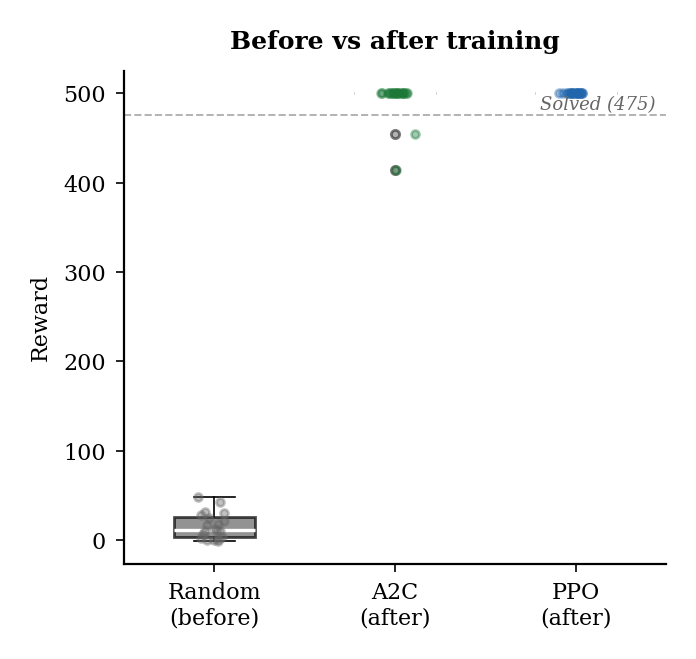
\includegraphics[width=0.42\textwidth]{results_task/fig5_before_after.png}
\caption{训练前后20回合评估奖励分布。PPO（蓝色）箱体压缩为单值500；A2C（绿色）中位数500但有3个异常值；随机策略（灰色）中位数约15分。}
\label{fig:before_after}
\end{figure}

\subsection{对比结果}

\textbf{总体性能排序。}如图\ref{fig:comparison}所示，五种控制方法的平均奖励排序为：\textbf{PPO（500.0）$>$ A2C（493.4）$\gg$ 规则控制器（215.8）$>$ LQR（44.8）$>$ 随机策略（16.1）}。PPO与A2C的均值差距仅1.4\%，但PPO标准差为0而A2C为20.8——稳定性差距显著。规则控制器是传统方法天花板，但仅达PPO性能的43.2\%。LQR仅比随机高约2.8倍。

\begin{figure}[H]
\centering
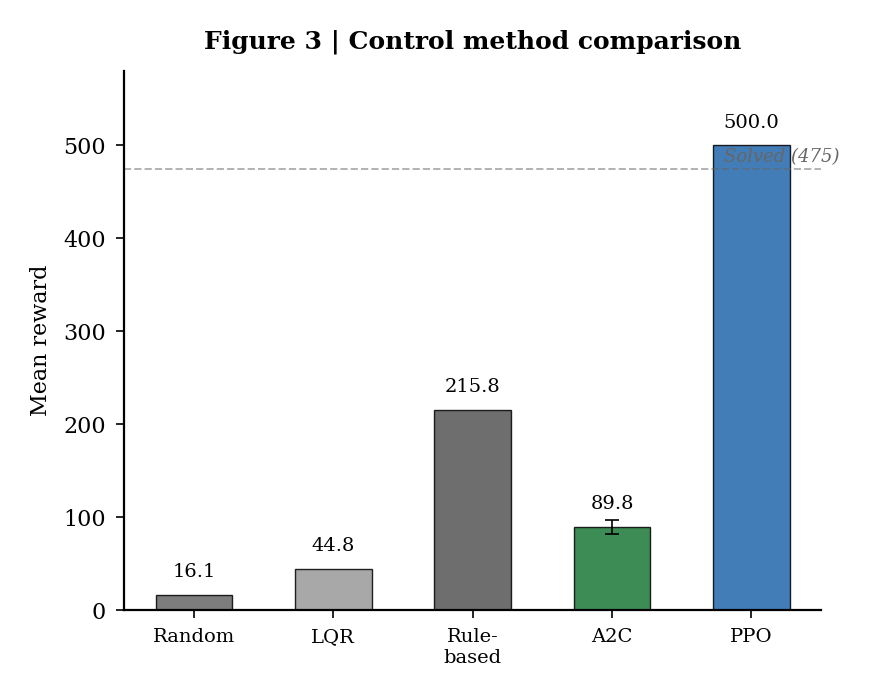
\includegraphics[width=0.50\textwidth]{results_task/fig3_method_comparison.png}
\caption{五种控制方法平均奖励对比（20回合评估，误差棒表示标准差）。}
\label{fig:comparison}
\end{figure}

\textbf{训练速度对比。}PPO首次满分在第280回合并持续保持，A2C首次满分在第400回合但波动频繁——PPO快约30\%。传统方法无需训练，但性能大幅折损。

\textbf{稳定性对比。}PPO标准差0（100\%可靠），A2C标准差20.8（90\%达标），规则控制器标准差29.1（最高但均值215.8）。

\begin{table}[H]
\centering
\caption{五种控制方法全面对比}
\label{tab:comparison}
\begin{tabular}{lccccc}
\toprule
\textbf{方法} & \textbf{平均奖励} & \textbf{标准差} & \textbf{达标率} & \textbf{训练步数} & \textbf{是否收敛} \\
\midrule
随机策略 & 16.1 & 6.8 & 0\% & 0 & 否 \\
LQR & 44.8 & 7.4 & 0\% & 0 & 否（模型失配） \\
规则控制 & 215.8 & 29.1 & 0\% & 0 & 否 \\
A2C（优化） & 493.4 & 20.8 & 90\% & 200,000 & 接近收敛 \\
\textbf{PPO} & \textbf{500.0} & \textbf{0.0} & \textbf{100\%} & \textbf{200,000} & \textbf{完全收敛} \\
\bottomrule
\end{tabular}
\end{table}

% ================================================================
\section{总结体会}

\textbf{算法效果总结。}PPO以满分500、零标准差完美解决问题，是唯一兼具高能力与高稳定性的算法。优化后的A2C（n\_steps=64, lr=5e-4）评估均值493.4、达标率90\%，性能接近PPO。传统控制方法中，规则控制器（215.8分）大幅超越LQR（44.8分）和随机策略（16.1分），证明了在强非线性系统中启发式规则的有效性。

\textbf{存在的问题与可改进方向。}（1）算法覆盖度不足：仅对比了PPO和A2C，可引入SAC、TD3等更先进的算法；（2）A2C稳定性不足：仍有10\%的评估回合失败，可尝试调整网络结构；（3）超参数搜索不充分：仅覆盖了n\_steps和学习率两个维度；（4）泛化性验证缺失：未测试物理参数变化时的鲁棒性；（5）训练效率：可引入课程学习加速训练。

\textbf{个人收获。}掌握了PPO和A2C两种主流RL算法的核心原理和实现差异，理解了超参数调优对RL算法性能的决定性影响——A2C从默认参数（后100均值41.2）到优化参数（后100均值464.5）的性能飞跃是最好的证明。认识到传统控制方法与RL方法的本质差异：前者依赖精确建模或人工规则，后者通过与环境试错交互自主学习策略。体会到了科学对比的重要性——多维度指标比单一均值能更全面地评估算法性能。

% ================================================================
\section{附录}

本项目代码已开源至GitHub，可从以下链接获取完整代码：

\href{https://github.com/zhaihuahua78/cartpole--}{https://github.com/zhaihuahua78/cartpole--}

\vspace{0.3cm}
\noindent\textit{报告完成日期：2026年7月}

\end{document}
